\section{Static Rankings in Detail}\label{app:static}
This appendix keeps the detailed static-ranking results of the evaluation (Section~\ref{sec:static}).
\subsection{How far the absolute-gradient default holds}\label{sec:default}
Table~\ref{tab:regret} reports the largest regret of every ranking in the decision-useful cells of each model and its resolved wins and losses against the absolute-gradient mask; Fig.~\ref{fig:map} in Appendix~\ref{app:evidence} shows the complete grid.

\begin{table}[t]
\caption{Decision-useful cells only. Left entry: largest regret against the best measured ranking in the same cell (accuracy points for classifiers, nats/token for language models). Right entry, $a$--$b$: cells in which the absolute-gradient mask is resolved better ($a$) or worse ($b$) than the listed ranking after Holm correction. FKeras was not measured on the transformers.}\label{tab:regret}
\centering\small
\begin{tabular}{l r@{\ \ }l r@{\ \ }l r@{\ \ }l r@{\ \ }l r@{\ \ }l}\toprule
 & \multicolumn{2}{c}{ResNet-8} & \multicolumn{2}{c}{DS-CNN} & \multicolumn{2}{c}{DistilBERT} & \multicolumn{2}{c}{Pythia} & \multicolumn{2}{c}{Qwen}\\
Ranking & \multicolumn{2}{c}{19 cells} & \multicolumn{2}{c}{22 cells} & \multicolumn{2}{c}{30 cells} & \multicolumn{2}{c}{17 cells} & \multicolumn{2}{c}{21 cells}\\\midrule
Absolute gradient & 0.06 & & 0.16 & & 0.14 & & 0.157 & & 0.035 &\\
Global gradient & 2.1 & 5--0 & 4.9 & 3--0 & 15.6 & 8--0 & 0.017 & 0--7 & 0.071 & 1--1\\
Positive gradient & 3.2 & 6--0 & 8.1 & 4--0 & 42.6 & 16--0 & 7.99 & 9--3 & 3.87 & 5--9\\
MSB-first & 12.7 & 6--0 & 3.4 & 2--0 & 34.5 & 11--0 & 1.18 & 11--1 & 1.73 & 11--0\\
FKeras & 12.7 & 7--0 & 2.2 & 2--0 & \multicolumn{2}{c}{---} & \multicolumn{2}{c}{---} & \multicolumn{2}{c}{---}\\
Numerical jump & 34.3 & 12--0 & 8.2 & 5--0 & 32.0 & 7--0 & 0.72 & 15--0 & 2.14 & 10--0\\
Random & 43.5 & 15--0 & 36.1 & 10--0 & 38.5 & 19--0 & 4.66 & 17--0 & 13.5 & 19--0\\\bottomrule
\end{tabular}
\Description{Maximum regret and resolved win-loss counts for seven rankings on five models.}
\end{table}
On the three classifiers the absolute-gradient mask is a clear default. Its regret never exceeds 0.16 accuracy points in a decision-useful cell and no other ranking is resolved better in any such cell, while every other ranking is resolved worse in 2 to 19 cells and loses up to 12.7 points (MSB-first, ResNet-8) or 42.6 points (positive gradient, DistilBERT). Where another letter appears in an unhatched classifier cell of Fig.~\ref{fig:map}, the difference is below 0.2 points and not resolved. On the language models the default is close to the best but not always the best. On Pythia the global-gradient mask is resolved better in seven of 17 decision-useful cells, by at most 0.157 nats per token, and on Qwen the two are equivalent within 0.07. In both, the absolute-gradient mask stays within a third of the usefulness margin of the best ranking, with the tight and loose margins as well.

\begin{table}[t]
\caption{Repeated evaluations of the classifiers (Section~\ref{sec:repeated}). Each replication has its own calibration draw, masks, input window and fault fields. Regrets are the largest accuracy loss, in points, against the best of the seven rankings in a decision-useful cell. The upper bound is the 95\% limit of the absolute-gradient mask's accuracy regret against any other ranking, with the replication as the unit, maximized over cells. Resolved contrasts use pooled fields with Holm correction. The retrained column gives the range over five copies of the reference recipe (resolved contrasts summed). All masks use 64 calibration inputs.}\label{tab:repeated}
\centering\footnotesize\setlength{\tabcolsep}{4pt}
\begin{tabular}{l r r r r r r}\toprule
 & \multicolumn{2}{c}{Pinned} & & Retrained & Pruned & Pruned \\
 & ResNet-8 & DS-CNN & Under-trained & ($\times$5) & 50\% & 70\%\\\midrule
Replications (fields per BER) & 9 (36) & 11 (88) & 8 (16) & 8 (16) each & 8 (16) & 8 (16)\\
Clean accuracy (\%) & 87.1 & 91.7 & 81.5 & 86.3--87.3 & 85.7 & 83.7\\
Decision-useful cells & 20 & 22 & 25 & 21--22 & 20 & 18\\
Absolute-gradient largest regret & 0.19 & 0.06 & 1.46 & 0.29--0.64 & 0.40 & 0.46\\
Largest upper bound & 0.64 & 0.20 & 2.47 & 1.00--1.93 & 2.24 & 1.36\\
Contrasts resolved for / against & 63 / 0 & 48 / 0 & 60 / 3 & 238 / 1 & 37 / 0 & 36 / 0\\
Cells where a ranking is better by $\ge$1 point & 0 & 0 & 3 & 0 & 0 & 0\\
MSB-first largest regret & 13.1 & 3.0 & 49.1 & 29.4--37.4 & 19.4 & 28.9\\
FKeras largest regret & 13.1 & 1.8 & 24.9 & 10.2--14.5 & 19.4 & 8.8\\
Highest useful BER, 12.5\% ($10^{-4}$), MSB / abs. & 10 / 30 & 30 / 30 & 10 / 100 & 3--10 / 30 & 10 / 30 & 3 / 10\\\bottomrule
\end{tabular}
\Description{Regrets, bounds and resolved contrasts of repeated evaluations on ResNet-8, DS-CNN, five retrained ResNet-8 copies and three further ResNet-8 checkpoints.}
\end{table}

These comparisons use one mask per ranking, one input window and one checkpoint per model. Table~\ref{tab:repeated} varies all three. On the pinned ResNet-8 and DS-CNN the default meets the rule fixed before the runs: with the replication as the unit, the upper bound on its regret against every other ranking stays below one point in every decision-useful cell (0.64 and 0.20 points), and no ranking is resolved better. On ResNet-8 at $p=3\times10^{-3}$ and 12.5\% its gain over MSB-first is 13.1 points (replication-level interval 9.4 to 16.8), against 12.7 in the main grid. On DS-CNN its margin over significance is modest: MSB-first and FKeras trail by at most 3.0 and 1.8 points. Appendix~\ref{app:repeated} shows the curves.

On five copies retrained from scratch with the reference recipe and on the pruned checkpoints the default also holds with 64-input masks. No ranking is better by a point in any decision-useful cell; its largest regret is 0.29 to 0.64 points on the retrained copies and 0.40 and 0.46 on the pruned checkpoints; and one of 239 resolved contrasts on the retrained copies goes against it, by less than a point. With eight replications the replication-level bounds reach 1.0 to 2.2 points. On the under-trained checkpoint the default does not hold: in three cells another ranking is better by more than a point (Section~\ref{sec:reversals}). Significance-first protection falls far behind on every checkpoint (Fig.~\ref{fig:fragility}). At $p=3\times10^{-3}$ and 12.5\% MSB-first loses 9 to 34 accuracy points across the nine ResNet-8 checkpoints, where the absolute gradient loses 0.6 to 5.3, and its largest regret ranges from 13.1 points on the pinned checkpoint to 49 on the under-trained one. On the retrained copies (29 to 37 points) this worst case is at a half-protected tier (18.75\%, $p=10^{-2}$) where the pinned checkpoint is not usable; at complete tiers the losses are similar.

\begin{figure}[tbp]
\centering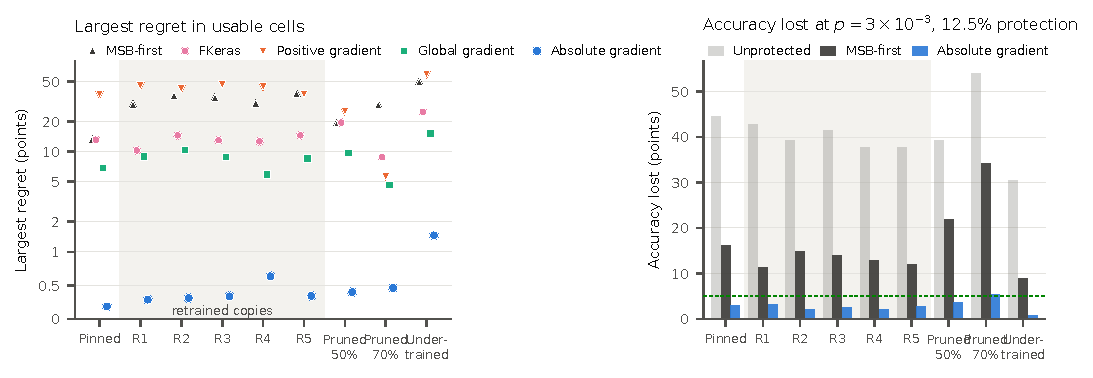
\includegraphics[width=\linewidth]{tecs_checkpoint_fragility}
\caption{The ResNet-8 checkpoints of Table~\ref{tab:repeated}: the pinned MLPerf reference, five copies retrained with its recipe (R1--R5), two pruned checkpoints and one under-trained checkpoint. Left: largest regret of each ranking in decision-useful cells (symmetric-log axis). Right: accuracy lost at $p=3\times10^{-3}$ and 12.5\% protection; the dashed line is the usefulness margin.}\label{fig:fragility}
\Description{Two panels comparing MSB-first, FKeras, gradient rankings and no protection across nine ResNet-8 checkpoints.}
\end{figure} These statements concern the seven rankings; search-based and literature-derived masks are compared in Section~\ref{sec:discussion}.

\subsection{When the preferred ranking changes}\label{sec:reversals}
The examples of Section~\ref{sec:allocation} show that the preferred ranking can depend on BER and budget. With masks built from 64 calibration inputs, this happens in the decision-useful region on the language models and on the under-trained ResNet-8; no pair of rankings shows resolved wins in both directions on the pinned or pruned ResNet-8, DS-CNN or ToyCar, and the single such pair on DistilBERT involves the random baseline. With more calibration inputs it happens on most ResNet-8 checkpoints.

On Pythia and Qwen the reversals are dominated by the positive-gradient ranking. It is the best measured ranking at the lowest BERs, by 0.01 to 0.03 nats per token over absolute gradient on Qwen at $p\le3\times10^{-4}$, and becomes worse by 0.2 to 1.1 nats per token at $3\times10^{-3}$ and by 3.8 at $10^{-2}$. What it gains where faults are sparse is two orders of magnitude smaller than what it loses where they are not.

On the under-trained ResNet-8 the same ranking produces a reversal that matters at both ends. At $p=10^{-3}$ the positive-gradient mask is better than the absolute-gradient mask by 1.3 accuracy points at 12.5\% protection (interval 1.0 to 1.7; 0.8 to 1.8 with the replication as the unit) and by 1.1 points at 25\%, both resolved after Holm correction. At $p=10^{-2}$ it is worse by 22.6 and 12.3 points. All four cells are decision-useful, so for this checkpoint no single static ranking is best across the useful band. At $10^{-3}$ the positive-gradient mask even leaves the model 1.2 points more accurate than it is without faults; Section~\ref{sec:harm} explains why.

The well-trained checkpoints hide the same reversal behind the calibration size (Appendix~\ref{app:calibration}). The positive score $\E_x\max(0,e_b)=\tfrac12(\E_x|e_b|+\E_x e_b)$ contains the mean effect $\E_x e_b$, whose per-input terms largely cancel, so 64 inputs estimate it poorly. With both masks built from 1,024 inputs, the positive-gradient mask is ahead at $10^{-3}$ in all 36 decision-useful cells of the nine checkpoints, by 0.2 to 1.6 points, and behind in all 15 at $10^{-2}$, by 0.6 to 17.8. Five checkpoints, the pinned one included, show resolved wins in both directions, and by the rule fixed before the runs the default does not hold at 512 or more inputs. Its own mask is settled at 64 inputs.

Two further effects are smaller: on Pythia at $p=3\times10^{-3}$ and 25\%, where it protects two complete tiers, MSB-first is better than absolute gradient by 0.09 nats per token, and within a half-protected tier structured fills beat a uniformly random one while FKeras does not beat storage order (Appendix~\ref{app:repeated}). Reversals outside the decision-useful region are not interpreted, and a bit-exact replay of every saved language-model field shows that the loss cap changes no conclusion in a decision-useful cell (Appendix~\ref{app:evidence}).

\subsection{Protection that is worse than none}\label{sec:harm}
Under ideal suppression a protected model receives a subset of the faults of the unprotected model, so it is tempting to assume that protection can only help. Figure~\ref{fig:harm} shows that it need not. With the positive-gradient mask, DistilBERT has a higher error rate than the unprotected model in six cells, by up to 6.0 points (interval 4.7 to 7.3, at $p=3\times10^{-2}$ and 6.25\%), and a higher loss in 17 of 32 cells; Pythia has a higher loss in eight cells, by up to 5.8 nats per token. Four of the DistilBERT accuracy cells are decision-useful: a designer who chose this ranking would have done worse than by protecting nothing, while the absolute-gradient mask keeps accuracy between 87\% and 90\% in the same cells. Checks for a defect in pairing, fault accounting, scores and nonfinite outputs found none (Appendix~\ref{app:harm}).

\begin{figure}[tbp]
\centering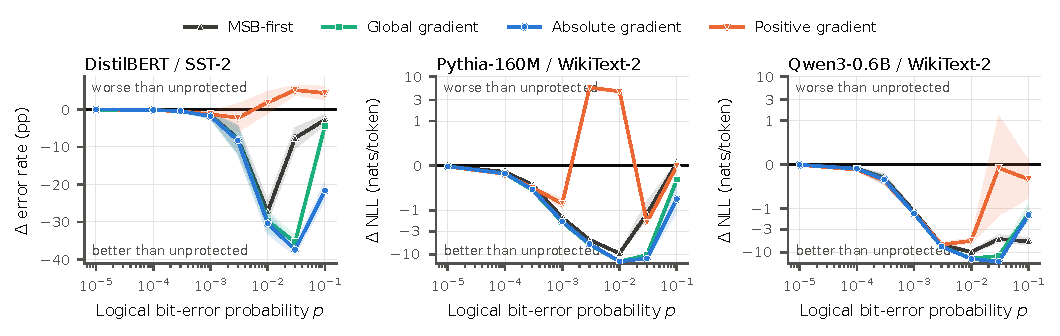
\includegraphics[width=\linewidth]{tecs_protection_vs_unprotected_125}
\caption{Paired difference between each protected model and the unprotected model on the same fault fields, at 12.5\% protection. Positive values mean protection made the task metric worse. Bands are 95\% paired intervals. The figure shows the three transformers, for which no FKeras ranking was measured.}\label{fig:harm}
\Description{Three panels showing that the positive-gradient mask becomes worse than no protection at intermediate bit-error probabilities.}
\end{figure}

The mechanism, obtained offline from the saved gradients, masks and stored codes of DistilBERT, is a one-sided remainder (Table~\ref{tab:drift} in Appendix~\ref{app:harm}). For every other mask the loss-increasing and loss-decreasing first-order effects of the unprotected bits cancel to within 0.5\%; the positive-gradient mask protects mainly loss-increasing flips, so the effects of what it leaves sum to $+6.7$ against $-20.6$. The many remaining faults then push the weights coherently in one direction, far beyond the range in which a gradient describes the loss. The amount of perturbation left is not the explanation: this mask leaves about the same squared jump size as the other gradient masks.

The under-trained ResNet-8 shows the same one-sided remainder with the opposite outcome at low fault rates. Its loss is not at a minimum, so a few faults pushed in the loss-decreasing direction act like a training step and raise accuracy above the clean model's; denser faults overshoot. A weaker form of this appears on the well-trained checkpoints once the positive score is estimated from more inputs (Appendix~\ref{app:calibration}). Its stored codes are distributed like those of the other checkpoints (Appendix~\ref{app:harm}), so the difference lies in where the weights sit on the loss surface, not in their values. Every ranking built from clean-model gradients assumes that the deployed model sits near a minimum, and a checkpoint that does not is one of the conditions under which a fixed ranking can mislead. The mechanism was checked directly for DistilBERT only.

